\documentclass{article}
\usepackage[left=2cm,right=2cm,top=3cm,bottom=3cm]{geometry}
\usepackage[polish]{babel}
%\usepackage[cp1250]{inputenc}
\usepackage{polski}
\usepackage{fancyhdr}
%\usepackage{amssymb}
%\usepackage[T1]{fontenc}
%\usepackage{lingmacros}
%\usepackage{tree-dvips}
\usepackage{graphicx}
\graphicspath{ {./img/} }
\usepackage{wrapfig}
\usepackage{array}
\usepackage{makecell}
%\renewcommand{\cellalign/theadalign}{vh}

\frenchspacing
\begin{document}
\pagestyle{fancy}
\fancyhead[LE,RO]{Mariusz Sendyk, Jakub Solich}
\fancyhead[LO,RE]{Mechatronika}
    \section{Cel projektu}
    Celem projektu jest zbudowanie klawiatury komputerowej w układzie
    ANSI TKL. Za pracę klawiatury odpowiadać będzie mikrokontroler, który zajmie się 
    komunikacją z komputerem poprzez USB.
    Głównym wyzwaniem projektu jest stworzenie kompletnego układu mikrokontrolera oraz programu
    w postaci modułu, do którego można będzie przyłączyć matrycę przycisków.

    \section{Założenia projektu}
    Na podstawowe założenia projektu składają się:
        \begin{itemize}
            \item Układ klawiatury w układzie ANSI TKL
            \item Komunikacja z komputerem poprzez USB
            \item Pooling rate 500Hz lub więcej
            \item Programowy de-bouncing
            \item Wspomaganie adresowania matrycy przełączników przy pomocy układów 74AHC138
            \item Wsparcie NKRO
        \end{itemize}
    Na dodatkowe założenia projektowe składają się:
        \begin{itemize}
            \item Obsługa makr
            \item Sterowanie podświetleniem poprzez moduł
            \item Mini system operacyjny
        \end{itemize}
    \section{Wybór rozwiązania projektowego}
    Praca klawiatury komputerowej w głównej mierze sprowadza się do ciągłego wykonywania następujących
    czynności przez mikrokontroler:
    \begin{enumerate}
        \item Pobierz stany przełączników (np. wykrycie stanu wysoki/niski na pinach)
        \item Na podstawie danych, wygeneruj kolejkę zmian przycisków (downstroke i upstroke, scancode)
        \item Prześlij dane do komputera/hosta
    \end{enumerate}
    Oczywiście to jest najsurowsza pętla pracy klawiatury. Jako układy wykonawczy postanowiono wykorzystać
    układ ATMega32U4. Jest to mikrokontroler firmy Atmel (obecnie pod Microchip), który jest szeroko stosowany
    w układach hobbystycznych. Układ ma ten następujące cechy, decydujące o jego zastosowanu:
    \begin{itemize}
        \item Duża wydajność obliczeniowa (głównie istrukcje wykonywane w 1 cyklu zegara oraz maks 16MHz)
        \item Sprzętowe USB dające sporo możliwości
        \item Bogate wyposarzenie tj. 4 liczniki,  I\textsuperscript{2}C, SPI, tryby uśpienia, 2 pełne 8-bitowe porty I/O
        \item Zintegrowany stabilizator 3,3V, wymagany dla komunikacji z USB
        \item Bogata dokumentacja i obecność gotowych rozwiązań OpenSource (GH60) opatych na tym układzie
        \item Przyjazna w lutowaniu obudowa TQFP44
        \item I przede wszystkim spora ilość projektów klawiatur OpenSource opartych na tym układzie
    \end{itemize}
    Wybrany mikrokontroler posiada 44 piny. Standardowy układ ANSI posiada 104 klawisze. Z góry widać, że bezpośrednie
    podłączenie przysków do pinów mikrokontrolera nie wystarczy. Zamiast takiego podejścia stosuje się \emph{matrycę przełączników}.
    \newpage
    \begin{figure}
        \centering
        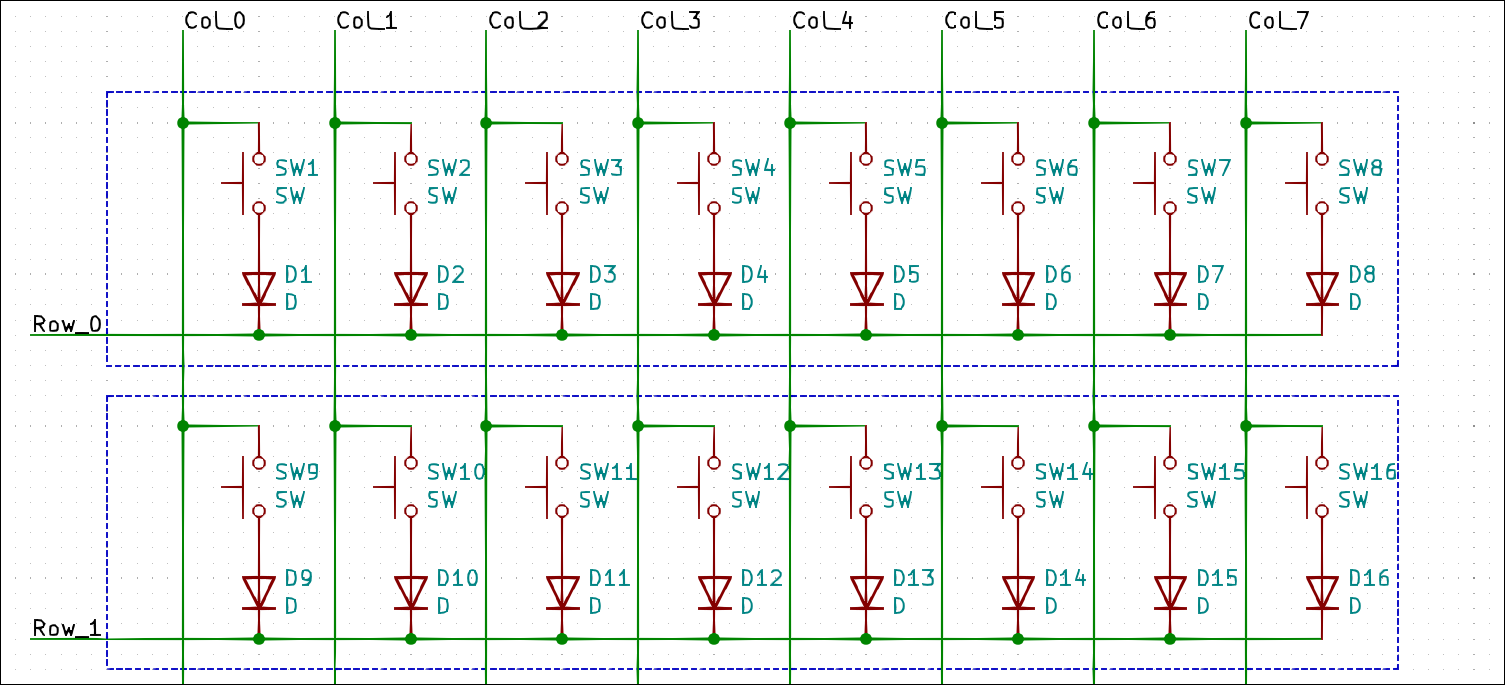
\includegraphics[width=\textwidth]{1}
    \end{figure}
    Połączenie przełączników w matrycę pozwala na adresowanie wybranej kolumny przycisków, a następnie ich odczytu.
    Ponieważ podczas odczytu musi być aktywna tylko jedna kolumna, to atrakcyjnym jest zastosowanie dekoderów n do n\textsuperscript{2}.
    Przykładowymi układami mogą być 74HC154 lub 74AHC138. Pierwszy układ to dekoder 4-do-16, zamienia 4 bitową wartość
    na wejściach na 1 z 16 na wyjściach. Aktywne wyjście przyjmuje stan niski, co pozwala na zastosowanie go bezpośrednio w układzie.
    Układ 74AHC138 jest tym samym układem co 154, ale 3-do-8. Oba układy posiadają możliwość łączenia w celu rozszerzenia
    ilości linii. Układ 154 byłby idealny, ponieważ 8*16 daje 128 klawiszy. Niestety, układ ten jest już stary 
    i dostępny jedynie w starym procesie technologicznym HC(T), który posiada duże opóźnienia (mogą one przekroczyć 
    50ns) i pobiera więcej energii (chociaż i tak pobierana energia jest znikoma). 74AHC138 natomiast, jest dostępny
    w procesie AHC, który jest znacznie szybszy (wszelkie opóźnienia nie przekraczają 10ns) i łatwiej dostępny.
    Układ ten również można rozszerzyć do 5-do-32. W naszym przypadku jedynie potrzebne jest 16 linii, ale nic nie
    stoi na przeszkodzie, by układ rozubodwać.
    
    \begin{center}
        \begin{tabular}{ |c|c|c|c|c| }
            \hline
            \thead{Oznaczenie} & \thead{Opis} & \thead{Tpd} & \thead{Tt} & \thead{Warunki\\An do Qn}  \\ 
            \hline
            74HC4515 & \makecell{4-to-16 line decoder/demultiplexer with input latches;inverting} & 50ns & 15ns  & \makecell{4,5V}  \\
            \hline
            74HC154 & \makecell{4-to-16 line decoder/demultiplexer} & 30ns & 15ns  & \makecell{4,5V}  \\ 
            \hline
            74AHC138 & \makecell{3-to-8 line decoder/demultiplexer; inverting} & 10.1ns & N/A  & \makecell{4,5-5,5V} \\
            \hline
        \end{tabular}
    \end{center}
    \begin{figure}
        \centering
        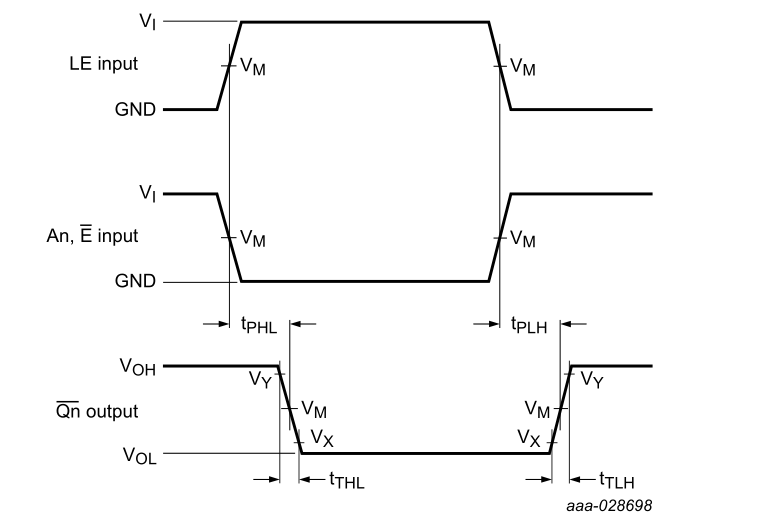
\includegraphics[width=0.4\textwidth]{2}
    \end{figure}
    \begin{center}
        \begin{tabular}{ |c|c|c|c|c|c|c|c|c| }
            \hline
            \thead{Producent} & \thead{SKU} & \thead{n-pin} & \thead{Flash} & \thead{SRAM} & \thead{EEPROM} & \thead{Wydajność} & \thead{Napięcie} & \thead{Peryferia}\\ 
            \hline
            Atmel/Microchip & ATMega32U4 & 44 & 32KB & 2,5KB & 1KB & 16MIPS & 2,7-5,5V & \makecell{USB\\JTAG\\SPI\\TWI\\USART\\ADC}\\
            \hline
            NXP & MC9S08JM60 & do 64 & do 60KB & do 4KB & N/A & 48MHz &  2,7-5,5V & \makecell{USB\\SPI\\TWI\\ADC\\RTC}\\ 
            \hline
            Microchip & PIC18F47J13 & 44 & 128KB & 3760B & N/A & 12MIPS & 2-3,6V & \makecell{USB\\SPI\\TWI\\RTCC\\ADC}\\
            \hline
        \end{tabular}
    \end{center}
\end{document}
